\newgeometry{left=7cm,right=3cm,
 marginparsep=15pt, marginparwidth=4.2cm,top=2cm}

\parindent0pt
\cxset{
 name=,
 numbering=none,
 number font-size=LARGE,
 number font-family=\rmfamily,
 number font-weight=\bfseries,
 number before={\parindent0pt },
 number dot=,
 number after=,
 number position=leftname,
 chapter font-family=,
 chapter font-weight=,
 chapter font-size=,
 chapter before=,
 chapter after=,
 chapter color=blue,
 number color=blue,
 title beforeskip={\parindent0pt},
 title afterskip={\vspace*{50pt}\par},
 title before={},
 title after={},
 title font-family=rmfamily,
 title font-color=black!80,
 title font-weight=normalfont,
 title font-size=Huge,
 title font-shape=itshape,
 chapter opening=any}
\chapter{Introduction to Style Fifteen}

\parindent1em
\def\thefigure{\arabic{chapter}.\arabic{figure}}
\lorem\par

\marginpar{%
 {\centering
 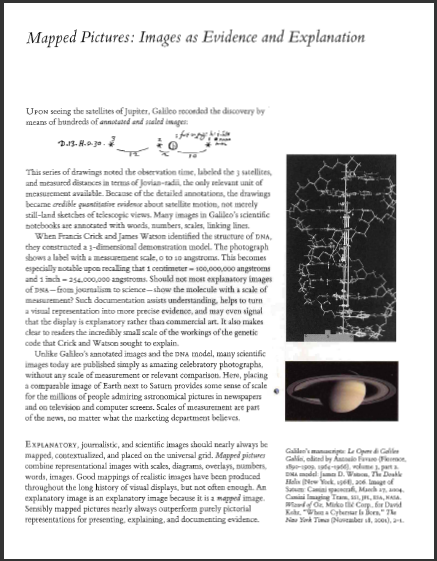
\includegraphics[width=4.2cm]{./chapters/chapter15.png}\vskip5pt\par}
 {\footnotesize\protect\lorem}
}
\marginpar{%
{\centering
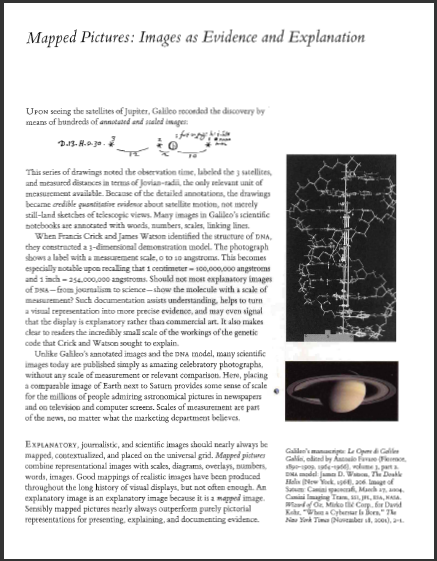
\includegraphics[width=4.2cm]{./chapters/chapter15.png}\par}
 
}

This is another marginpar of the same size.

\lorem

\lipsum
\marginpar{%
{\centering
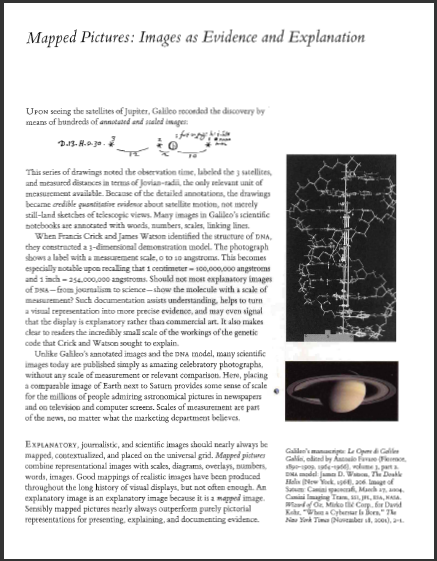
\includegraphics[width=4.2cm]{./chapters/chapter15.png}\par}
}

